%! Author = Sujal Singh
%! Date = 2/24/23


% Preamble
\documentclass[11pt]{article}

\title{\textbf{Critical Misconfiguration in the Firewall Rules of \\ Customer Intranet}}
\author{Sujal Singh \\ \href{mailto:contact@sujal.dev}{contact@sujal.dev}}
\date{}

\pagenumbering{gobble}
\twocolumn
\setlength{\columnsep}{25pt}

% Packages
\usepackage[letterpaper, total={7.2in, 9in}]{geometry}
\usepackage[hidelinks]{hyperref}
\usepackage[section]{placeins}
\usepackage{mathptmx}
\usepackage{graphicx}
\usepackage[outputdir=../output]{minted}
\usepackage{enumitem}
\usepackage{lipsum}

% Document
\begin{document}
    \maketitle

    \section*{Abstract}
    This report details a critical misconfiguration in the firewall rules of the local network of customers created by
    ACT Fibernet to share a single public IPv4 address with multiple customers behind a CGNAT.\ There exists no rule
    that blocks communication between two clients connected to this network.\ This is currently allowing customers
    belonging to a particular network to access each other's devices.

    \begin{figure}[!htb]
        \centering
        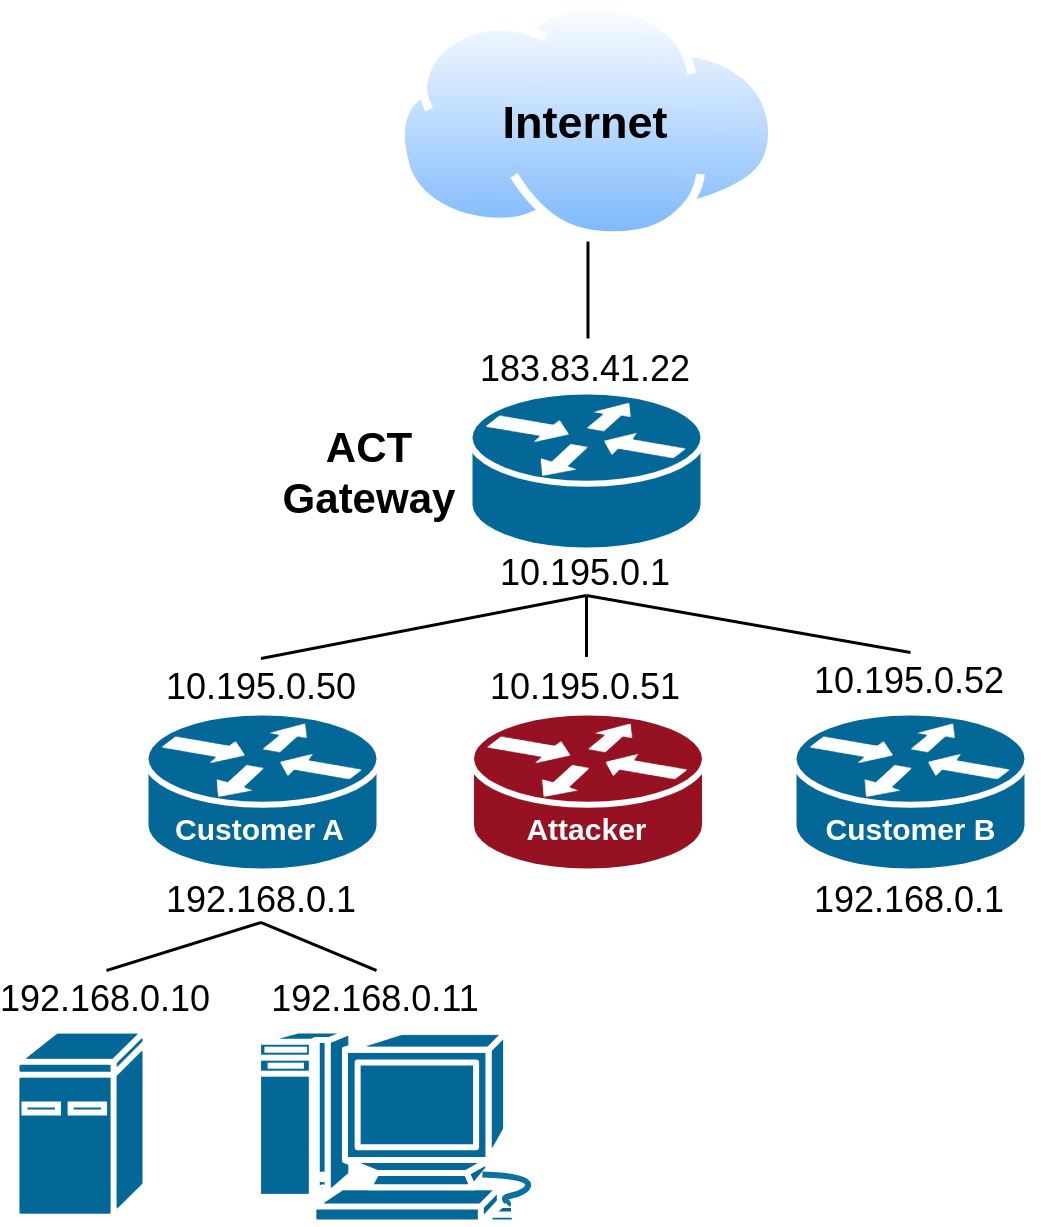
\includegraphics[width=140pt]{./diagrams/network-hierarchy}
        \caption{Customer Intranet}
        \label{fig:1}
    \end{figure}

    A malicious customer can gain access to any device on the network with a default password, or exploit any other
    vulnerability present in the device to gain access.\ Some routers distributed by ACT also have a default password
    of \emph{``act@123''}{.} Once an attacker gains access to a device such as the router, it will have control over
    the entire network of the target, allowing the attacker to carry out \textbf{several high severity attacks} such as
    DNS hijacking.\ All of this is easily preventable if ACT takes the necessary steps to fix the issue.


    \section{Steps to reproduce}\label{sec:steps-to-reproduce}
    A malicious customer can use any network scanner such as \emph{nmap} to discover vulnerable devices.\ But first
    one has to figure out a few parameters to begin scanning the network.
    \begin{enumerate}[leftmargin=*]
        \item Figure out your gateway's gateway, i.e, the gateway of the local network created by ACT.\ This can be done
        by running the following command (on a *nix machine):
        \begin{minted}[tabsize=0]{bash}
$ traceroute example.com
...
 2  10.195.0.1 (10.195.0.1)  4.526 ms  4.690 ms
...
        \end{minted}
        This is usually going to be the second hop in output, in this case it's \texttt{10.195.0.1}.\ This assumes that
        there exists a router between you and ACT's router and you're not directly plugging in the WAN cable coming
        to your home to the device you're using to run traceroute.

        \item One can now begin scanning the network by running the following (change the IP address according to
        the value received in the previous step):
        \begin{minted}[tabsize=0]{bash}
$ nmap -p 80 10.195.0.0-255
        \end{minted}
        In this example, I've chosen to only scan a small portion of the network with devices that have port 80 open
        so that the scan is fairly quick.\ A full network scan would take a very long time.
    \end{enumerate}


    \section{Impact}\label{sec:impact}
    Depending on what kind of device one is able to access via this technique, there are various highly severe threats
    posed by this.

    \subsection{Routers}\label{subsec:routers}
    An attacker will easily be able to access routers with default passwords, giving the attacker various information
    such as the WiFI password and SSID, hostnames of the hosts connected to the LAN, etc.\

    \subsubsection{DNS Hijacking}
    An attacker can configure a malicious DNS server to be advertised via DHCP on the target's router, allowing it
    direct any domain to any IP address.\ The attacker could also simply just monitor which sites a user visits,
    which violates the privacy of the target.

    \subsubsection{Phishing}
    Having control over the DNS server will allow the attacker to employ phishing attacks on the target, including
    but not limited to net \textbf{banking sites, email, other such critical services.}

    \subsubsection{Fake CA Certificate}
    Once the attacker has configured a malicious DNS servers it can redirect the target to a fake warning page which
    employs various social engineering techniques to manipulate the user into installing a CA certificate owned by the
    attacker.

    \subsubsection{Man in the Middle}
    Having control over the DNS server and having a fake CA certificate installed on the target's machine, the
    attacker can now MITM all traffic, including encrypted traffic.\ The possibilities here are endless.

    \subsubsection{PPPoE Credentials}
    The attacker might be able to figure out the \textbf{name, email, mobile number, address} of the target.\ The
    attacker can obtain the PPPoE credentials of the target by accessing the target's router.\ Feeding bogus PPPoE
    credentials to target's router so that there is no conflict for the next step.\
    Visiting \href{https://selfcare.actcorp.in}{selfcare.actcorp.in} and logging in with the obtained credentials
    will reveal the aforementioned information.

    \subsection{CCTV Cameras}\label{subsec:cctv-cameras}
    An attacker can gain access to CCTV cameras having default passwords (which is fairly common) connected to the
    network.\ One can monitor, control, disable the camera without the target having any idea.\ Needles to say this
    is a giant breach into the target's privacy and could also have real world consequences, such as disabling a camera
    during a robbery.


    \section{Proposed Solution}\label{sec:proposed-solution}
    The solution to this problem is fairly straightforward.\ ACT Fibernet could setup a firewall rule disallowing
    client-to-client communication on that network since it does not serve any purpose at all and exposes the network
    to a plethora of attacks.\ Even if two clients need to communicate with each other on this intranet for whatever
    reason, a simple exception rule could be setup after assigning both of those clients a private static IP\@.

\end{document}